\PassOptionsToPackage{unicode}{hyperref}
\documentclass{beamer}

% --- Налаштування мови та шрифтів ---
\usepackage[T2A]{fontenc}
\usepackage[utf8]{inputenc}
\usepackage[ukrainian]{babel}
\usepackage{graphicx}
\usepackage{amsmath, amssymb, amsthm}

% Фікс для математичних шрифтів
\usefonttheme[onlymath]{serif}

% --- ТЕМА ТА КОЛЬОРИ ---
\usetheme{Berlin}
\usecolortheme{seahorse}

% --- НАЛАШТУВАННЯ КОЛЬОРІВ БЛОКІВ ---
\setbeamercolor{block title}{fg=white, bg=blue!80!black}
\setbeamercolor{block body}{fg=black, bg=blue!10}
\setbeamercolor{block title example}{fg=white, bg=green!50!black}
\setbeamercolor{block body example}{fg=black, bg=green!10}
\setbeamercolor{block title alert}{fg=white, bg=red!70!black}
\setbeamercolor{block body alert}{fg=black, bg=red!10}

\setbeamercolor{normal text}{fg=black}
\setbeamerfont{block title}{series=\bfseries}

% --- ПІДПИСИ ДО РИСУНКІВ ---
\setbeamertemplate{caption}[numbered]
\setbeamertemplate{caption label separator}{. }
\addto\captionsukrainian{\renewcommand{\figurename}{Рис.}}

% --- ДАНІ ТИТУЛЬНОГО СЛАЙДА ---
\title[Похідна функції]{Похідна функції}
\subtitle{Поняття, правила знаходження та застосування}
\author[Прізвище І.П.]{Миколаєнко Дмитро}
\institute[ФМФ]{Факультет математики, фізики та комп'ютерних наук}
\date{\today}

\begin{document}

% 1. ТИТУЛЬНИЙ СЛАЙД
\begin{frame}
    \titlepage
\end{frame}

% 2. ЗМІСТ
\begin{frame}{План презентації}
    \tableofcontents
\end{frame}

% 3. ВСТУП
\section{Загальні відомості}
\begin{frame}{Що таке похідна?}
    \begin{block}{Означення}
        Похідною функції $f(x)$ у точці $x_0$ називається границя відношення приросту функції до приросту аргументу, якщо ця границя існує:
        \[
        f'(x_0)=\lim_{\Delta x \to 0}\frac{f(x_0+\Delta x)-f(x_0)}{\Delta x}.
        \]
    \end{block}

    \begin{itemize}
        \item Похідна характеризує швидкість зміни функції.
        \item Вона показує, як змінюється значення функції при зміні аргументу.
    \end{itemize}
\end{frame}

% 4. ГЕОМЕТРИЧНИЙ ЗМІСТ
\section{Теоретичні основи}
\begin{frame}{Геометричний зміст похідної}
    \begin{block}{Твердження}
        Похідна функції в точці дорівнює кутовому коефіцієнту дотичної до графіка функції в цій точці.
    \end{block}

    \begin{exampleblock}{Формула}
        Якщо дотична утворює з додатним напрямом осі $Ox$ кут $\alpha$, то
        \[
        f'(x_0)=k=\tan \alpha.
        \]
    \end{exampleblock}

    \begin{alertblock}{Увага}
        Похідна існує не в кожній точці. Якщо графік має кут або розрив, похідна може не існувати.
    \end{alertblock}
\end{frame}

% 5. ОСНОВНІ ПРАВИЛА
\begin{frame}{Основні правила диференціювання}
    \begin{block}{Правила}
        Якщо $u(x)$ і $v(x)$ — диференційовні функції, то:
        \[
        (u+v)'=u'+v'
        \]
        \[
        (u-v)'=u'-v'
        \]
        \[
        (uv)'=u'v+uv'
        \]
        \[
        \left(\frac{u}{v}\right)'=\frac{u'v-uv'}{v^2}, \quad v \ne 0
        \]
    \end{block}
\end{frame}

% 6. ПОХІДНІ ЕЛЕМЕНТАРНИХ ФУНКЦІЙ
\begin{frame}{Похідні елементарних функцій}
    \begin{exampleblock}{Основні формули}
        \[
        (C)'=0
        \]
        \[
        (x^n)'=nx^{n-1}
        \]
        \[
        (\sin x)'=\cos x
        \]
        \[
        (\cos x)'=-\sin x
        \]
        \[
        (e^x)'=e^x
        \]
        \[
        (\ln x)'=\frac{1}{x}
        \]
    \end{exampleblock}
\end{frame}

% 7. ТЕОРЕМА
\begin{frame}{Необхідна умова екстремуму}
    \begin{block}{Теорема Ферма}
        Якщо функція $f(x)$ має в точці $x_0$ локальний максимум або локальний мінімум і в цій точці існує похідна, то
        \[
        f'(x_0)=0.
        \]
    \end{block}

    \begin{itemize}
        \item Ця теорема допомагає знаходити критичні точки.
        \item Через критичні точки досліджують функцію на зростання і спадання.
    \end{itemize}
\end{frame}

% 8. ПРИКЛАД
\section{Приклади}
\begin{frame}{Приклад знаходження похідної}
    \begin{exampleblock}{Знайти похідну функції}
        \[
        y = x^3 - 4x^2 + 2x + 1
        \]
    \end{exampleblock}

    \begin{align*}
        y' &= (x^3)' - (4x^2)' + (2x)' + (1)' \\
           &= 3x^2 - 8x + 2
    \end{align*}

    Отже,
    \[
    y' = 3x^2 - 8x + 2.
    \]
\end{frame}

% 9. ГРАФІКА
\section{Візуалізація}
\begin{frame}{Графік функції та дотична}
    \begin{columns}
        \begin{column}{0.52\textwidth}
            Похідна пов’язана з дотичною до графіка функції.

            \begin{itemize}
                \item Якщо $f'(x)>0$, функція зростає.
                \item Якщо $f'(x)<0$, функція спадає.
                \item Якщо $f'(x)=0$, можлива критична точка.
            \end{itemize}
        \end{column}

        \begin{column}{0.48\textwidth}
            \begin{figure}
                \centering
                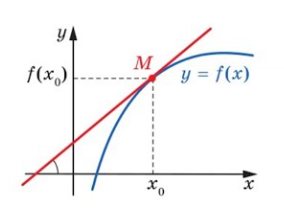
\includegraphics[width=0.9\textwidth]{foto1.png}
                \caption{Графік функції та дотична}
            \end{figure}
        \end{column}
    \end{columns}
\end{frame}

% 10. ЗАСТОСУВАННЯ
\section{Практичне значення}
\begin{frame}{Де застосовується похідна?}
    \begin{enumerate}
        \item У фізиці — для знаходження швидкості та прискорення.
        \item В економіці — для аналізу прибутку, витрат і продуктивності.
        \item У техніці — для моделювання процесів.
        \item У математиці — для дослідження функцій.
    \end{enumerate}

    \begin{block}{Висновок}
        Похідна є одним з найважливіших понять математичного аналізу, яке має велике теоретичне та практичне значення.
    \end{block}
\end{frame}

% 11. ЗАКЛЮЧНИЙ СЛАЙД
\section{Висновки}
\begin{frame}{Висновки}
    \begin{itemize}
        \item Розглянуто означення похідної.
        \item Наведено геометричний зміст похідної.
        \item Подано основні правила диференціювання.
        \item Розглянуто приклад знаходження похідної.
        \item Показано практичне застосування похідної.
    \end{itemize}

    \vspace{0.5cm}
    \centering
    \textbf{\Large Дякую за увагу!}
\end{frame}

\end{document}